%-----------------------------------------------------------------------------------------------------
%        روش اجرا.: 2 بار F1 ، 2 بار  F11(به منظور تولید مراجع) ، دوبار Ctrl+Alt+I (به منظور تولید نمایه) و دو بار F1 -------> مشاهده Pdf
%%%%%%%%%%%%%%%%%%%%%%%%%%%%%%%%%%%%%%%%%%%%%%%%%%%%%%
%   TeXstudio as your IDE
%%  برای compile در TeXstudio تنها کافی است منوی Options->Configure TeXstudio را زده و در پنجره Configure TeXstudio در بخش Build گزینه Default Compiler را به XeLaTeX تغییر دهید. سند شما به راحتی compile خواهد شد.
%   F1 & F5 : Build & view
%   F6      : Compile
%   F7      : View
%   --------------
%%%%%%%%%%%%%%%%%%%%%%%%%%%%%%%%%%%%%%%%%%%%%%%%%%%%%%
%        اگر قصد نوشتن رساله دکتری را دارید، در خط زیر به جای msc،
%      کلمه phd را قرار دهید. کلیه تنظیمات لازم، به طور خودکار، اعمال می‌شود.
\documentclass[fleqn,oneside,msc,12pt]{AUTthesis}
%       فایل commands.tex را حتماً به دقت مطالعه کنید؛ چون دستورات مربوط به فراخوانی بسته زی‌پرشین 
%       و دیگر بسته‌ها و ... در این فایل قرار دارد و بهتر است که با نحوه استفاده از آنها آشنا شوید. توجه شود برای نسخه نهایی پایان‌نامه حتماً hyperref را 
%        غیرفعال کنید.


% در این فایل، دستورها و تنظیمات مورد نیاز، آورده شده است.
%-------------------------------------------------------------------------------------------------------------------
% در ورژن جدید زی‌پرشین برای تایپ متن‌های ریاضی، این سه بسته، حتماً باید فراخوانی شود.
\usepackage{amsthm,amssymb,amsmath,amsfonts}
% بسته‌ای برای تنطیم حاشیه‌های بالا، پایین، چپ و راست صفحه
\usepackage[top=30mm, bottom=30mm, left=25mm, right=30mm]{geometry}
% بسته‌‌ای برای ظاهر شدن شکل‌ها و تصاویر متن
\usepackage{graphicx}
\usepackage{caption}
\usepackage{color}
%بسته‌ای برای تنظیم فاصله عمودی خط‌های متن
\usepackage{setspace}
\usepackage{indentfirst}
\usepackage{titletoc}
\usepackage{tocloft}
%با فعال کردن بسته زیر فوت‌نوت‌ها در هر صفحه ریست می‌شوند. حالت پیش‌فرض آن ریست شدن در هر فصل می‌باشد.
%\usepackage[perpage]{footmisc}
\usepackage{enumitem}
%\usepackage{titlesec}
% بسته‌ و دستوراتی برای ایجاد لینک‌های رنگی با امکان جهش
\usepackage[pagebackref=false,colorlinks,linkcolor=black,citecolor=black]{hyperref}
\usepackage[nameinlink]{cleveref}%capitalize,,noabbrev
 \AtBeginDocument{%
    \crefname{equation}{برابری}{equations}%
    \crefname{chapter}{فصل}{chapters}%
    \crefname{section}{بخش}{sections}%
    \crefname{appendix}{پیوست}{appendices}%
    \crefname{enumi}{مورد}{items}%
    \crefname{footnote}{زیرنویس}{footnotes}%
    \crefname{figure}{شکل}{figures}%
    \crefname{table}{جدول}{tables}%
    \crefname{theorem}{قضیه}{theorems}%
    \crefname{lemma}{لم}{lemmas}%
    \crefname{corollary}{نتیجه}{corollaries}%
    \crefname{proposition}{گزاره}{propositions}%
    \crefname{definition}{تعریف}{definitions}%
    \crefname{result}{نتیجه}{results}%
    \crefname{example}{مثال}{examples}%
    \crefname{remark}{نکته}{remarks}%
    \crefname{note}{یادداشت}{notes}%
}
% چنانچه قصد پرینت گرفتن نوشته خود را دارید، خط بالا را غیرفعال و  از دستور زیر استفاده کنید چون در صورت استفاده از دستور زیر‌‌، 
% لینک‌ها به رنگ سیاه ظاهر خواهند شد که برای پرینت گرفتن، مناسب‌تر است
%\usepackage[pagebackref=false]{hyperref}
% بسته‌ لازم برای تنظیم سربرگ‌ها
\usepackage{fancyhdr}
% بسته‌ای برای ظاهر شدن «مراجع»  در فهرست مطالب
\usepackage[nottoc]{tocbibind}
% دستورات مربوط به ایجاد نمایه
\usepackage{makeidx,multicol}
\setlength{\columnsep}{1.5cm}

%%%%%%%%%%%%%%%%%%%%%%%%%%
\usepackage{verbatim}
\makeindex
\usepackage{sectsty}
% فراخوانی بسته زی‌پرشین و تعریف قلم فارسی و انگلیسی
\usepackage{xepersian}%[extrafootnotefeatures]
\SepMark{-}
%حتماً از تک لایو 2014 استفاده کنید.
\settextfont[Scale=1.2]{B-NAZANIN.TTF}
\setlatintextfont{times new roman.ttf}
\renewcommand{\labelitemi}{$\bullet$}
%%%%%%%%%%%%%%%%%%%%%%%%%%
% چنانچه می‌خواهید اعداد در فرمول‌ها، انگلیسی باشد، خط زیر را غیرفعال کنید.
%در غیر اینصورت حتماً فونت PGaramond را نصب کنید.
%\setdigitfont[Scale=1.1]{Garamond.ttf}%%Yas
%%%%%%%%%%%%%%%%%%%%%%%%%%
% تعریف قلم‌های فارسی اضافی برای استفاده در بعضی از قسمت‌های متن
\defpersianfont\nastaliq[Scale=2]{IranNastaliq.ttf}
\defpersianfont\chapternumber[Scale=3]{B-NAZANIN.TTF}
%\chapterfont{\centering}%
%%%%%%%%%%%%%%%%%%%%%%%%%%
% دستوری برای تغییر نام کلمه «اثبات» به «برهان»
\renewcommand\proofname{\textbf{برهان}}

% دستوری برای تغییر نام کلمه «کتاب‌نامه» به «منابع و مراجع«
\renewcommand{\bibname}{منابع و مراجع}


% Headings for every page of ToC, LoF and Lot
\setlength{\cftbeforetoctitleskip}{-1.2em}
\setlength{\cftbeforelottitleskip}{-1.2em}
\setlength{\cftbeforeloftitleskip}{-1.2em}
\setlength{\cftaftertoctitleskip}{-1em}
\setlength{\cftafterlottitleskip}{-1em}
\setlength{\cftafterloftitleskip}{-1em}
%%\makeatletter
%%%%\renewcommand{\l@chapter}{\@dottedtocline{1}{1em\bfseries}{1em}}
%%%%\renewcommand{\l@section}{\@dottedtocline{2}{2em}{2em}}
%%%%\renewcommand{\l@subsection}{\@dottedtocline{3}{3em}{3em}}
%%%%\renewcommand{\l@subsubsection}{\@dottedtocline{4}{4em}{4em}}
%%%%\makeatother


\newcommand\tocheading{\vspace{1cm}\par عنوان\hfill صفحه \par}
\newcommand\lofheading{\vspace{1cm}\hspace*{.5cm}\figurename\hfill صفحه \par}
\newcommand\lotheading{\vspace{1cm}\hspace*{.5cm}\tablename\hfill صفحه \par}

\renewcommand{\cftchapleader}{\cftdotfill{\cftdotsep}}
\renewcommand{\cfttoctitlefont}{\hspace*{\fill}\LARGE\bfseries}%\Large
\renewcommand{\cftaftertoctitle}{\hspace*{\fill}}
\renewcommand{\cftlottitlefont}{\hspace*{\fill}\LARGE\bfseries}%\Large
\renewcommand{\cftafterlottitle}{\hspace*{\fill}}
\renewcommand{\cftloftitlefont}{\hspace*{\fill}\LARGE\bfseries}
\renewcommand{\cftafterloftitle}{\hspace*{\fill}}

%%%%%%%%%%%%%%%%%%%%%%%%%%
% تعریف و نحوه ظاهر شدن عنوان قضیه‌ها، تعریف‌ها، مثال‌ها و ...
%برای شماره گذاری سه تایی قضیه ها
\theoremstyle{definition}
\newtheorem{definition}{تعریف}[section]
\newtheorem{remark}[definition]{نکته}
\newtheorem{note}[definition]{یادداشت}
\newtheorem{example}[definition]{نمونه}
\newtheorem{question}[definition]{سوال}
\newtheorem{remember}[definition]{یاداوری}
\theoremstyle{theorem}
\newtheorem{theorem}[definition]{قضیه}
\newtheorem{lemma}[definition]{لم}
\newtheorem{proposition}[definition]{گزاره}
\newtheorem{corollary}[definition]{نتیجه}
%%%%%%%%%%%%%%%%%%%%%%%%
%%%%%%%%%%%%%%%%%%%
%%% برای شماره گذاری چهارتایی قضیه ها و ...
%%\newtheorem{definition1}[subsubsection]{تعریف}
%%\newtheorem{theorem1}[subsubsection]{قضیه}
%%\newtheorem{lemma1}[subsubsection]{لم}
%%\newtheorem{proposition1}[subsubsection]{گزاره}
%%\newtheorem{corollary1}[subsubsection]{نتیجه}
%%\newtheorem{remark1}[subsubsection]{نکته}
%%\newtheorem{example1}[subsubsection]{مثال}
%%\newtheorem{question1}[subsubsection]{سوال}

%%%%%%%%%%%%%%%%%%%%%%%%%%%%

% دستورهایی برای سفارشی کردن صفحات اول فصل‌ها
\makeatletter
\newcommand\mycustomraggedright{%
 \if@RTL\raggedleft%
 \else\raggedright%
 \fi}
\def\@makechapterhead#1{%
\thispagestyle{style1}
\vspace*{20\p@}%
{\parindent \z@ \mycustomraggedright
\ifnum \c@secnumdepth >\m@ne
\if@mainmatter

\bfseries{\Huge \@chapapp}\small\space {\chapternumber\thechapter}
\par\nobreak
\vskip 0\p@
\fi
\fi
\interlinepenalty\@M 
\Huge \bfseries #1\par\nobreak
\vskip 120\p@

}

%\thispagestyle{empty}
\newpage}
\bidi@patchcmd{\@makechapterhead}{\thechapter}{\tartibi{chapter}}{}{}
\bidi@patchcmd{\chaptermark}{\thechapter}{\tartibi{chapter}}{}{}
\makeatother

\pagestyle{fancy}
\renewcommand{\chaptermark}[1]{\markboth{\chaptername~\tartibi{chapter}: #1}{}}

\fancypagestyle{style1}{
\fancyhf{} 
\fancyfoot[c]{\thepage}
\fancyhead[R]{\leftmark}%
\renewcommand{\headrulewidth}{1.2pt}
}


\fancypagestyle{style2}{
\fancyhf{}
\fancyhead[R]{چکیده}
\fancyfoot[C]{\thepage{}}
\renewcommand{\headrulewidth}{1.2pt}
}

\fancypagestyle{style3}{%
  \fancyhf{}%
  \fancyhead[R]{فهرست نمادها}
  \fancyfoot[C]{\thepage}%
  \renewcommand{\headrulewidth}{1.2pt}%
}

\fancypagestyle{style4}{%
  \fancyhf{}%
  \fancyhead[R]{فهرست جداول}
  \fancyfoot[C]{\thepage}%
  \renewcommand{\headrulewidth}{1.2pt}%
}

\fancypagestyle{style5}{%
  \fancyhf{}%
  \fancyhead[R]{فهرست اشکال}
  \fancyfoot[C]{\thepage}%
  \renewcommand{\headrulewidth}{1.2pt}%
}

\fancypagestyle{style6}{%
  \fancyhf{}%
  \fancyhead[R]{فهرست مطالب}
  \fancyfoot[C]{\thepage}%
  \renewcommand{\headrulewidth}{1.2pt}%
}

\fancypagestyle{style7}{%
  \fancyhf{}%
  \fancyhead[R]{نمایه}
  \fancyfoot[C]{\thepage}%
  \renewcommand{\headrulewidth}{1.2pt}%
}

\fancypagestyle{style8}{%
  \fancyhf{}%
  \fancyhead[R]{منابع و مراجع}
  \fancyfoot[C]{\thepage}%
  \renewcommand{\headrulewidth}{1.2pt}%
}
\fancypagestyle{style9}{%
  \fancyhf{}%
  \fancyhead[R]{واژه‌نامه‌ی فارسی به انگلیسی}
  \fancyfoot[C]{\thepage}%
  \renewcommand{\headrulewidth}{1.2pt}%
}
%


%دستور حذف نام لیست تصاویر و لیست جداول از فهرست مطالب
\newcommand*{\BeginNoToc}{%
  \addtocontents{toc}{%
    \edef\protect\SavedTocDepth{\protect\the\protect\value{tocdepth}}%
  }%
  \addtocontents{toc}{%
    \protect\setcounter{tocdepth}{-10}%
  }%
}
\newcommand*{\EndNoToc}{%
  \addtocontents{toc}{%
    \protect\setcounter{tocdepth}{\protect\SavedTocDepth}%
  }%
}
\newcounter{savepage}
\renewcommand{\listfigurename}{فهرست اشکال}
\renewcommand{\listtablename}{فهرست جداول}
%\renewcommand\cftsecleader{\cftdotfill{\cftdotsep}}
%%%%%%%%%%%%%%%%%%%%%%%%%%%%%
%%%%%%%%%%%%%%%%%%%%%%%%%%%%

\begin{document}
\baselineskip=.75cm
\linespread{1.75}
%% -!TEX root = AUTthesis.tex
% در این فایل، عنوان پایان‌نامه، مشخصات خود، متن تقدیمی‌، ستایش، سپاس‌گزاری و چکیده پایان‌نامه را به فارسی، وارد کنید.
% توجه داشته باشید که جدول حاوی مشخصات پروژه/پایان‌نامه/رساله و همچنین، مشخصات داخل آن، به طور خودکار، درج می‌شود.
%%%%%%%%%%%%%%%%%%%%%%%%%%%%%%%%%%%%
% دانشکده، آموزشکده و یا پژوهشکده  خود را وارد کنید
\faculty{دانشکده مهندسی کامپیوتر}
% گرایش و گروه آموزشی خود را وارد کنید
\department{محل کارآموزی: شرکت عصرگویش‌پرداز}
% عنوان پایان‌نامه را وارد کنید
%\fatitle{مقدمه ای بر تشخیص خشونت در نظارت ویدیویی به کمک یادگیری عمیق}
% نام استاد(ان) راهنما را وارد کنید
\firstsupervisor{دکتر احمد نیک آبادی}
\secondsupervisor{}
% نام استاد(دان) مشاور را وارد کنید. چنانچه استاد مشاور ندارید، دستور پایین را غیرفعال کنید.
%\firstadvisor{نام کامل استاد مشاور}
%\secondadvisor{استاد مشاور دوم}
% نام نویسنده را وارد کنید
\name{امیرمحمد}
% نام خانوادگی نویسنده را وارد کنید
\surname{بابائی}
%%%%%%%%%%%%%%%%%%%%%%%%%%%%%%%%%%
\thesisdate{تابستان ۱۴۰۱}

% چکیده پایان‌نامه را وارد کنید
\fa-abstract{}


% کلمات کلیدی پایان‌نامه را وارد کنید
\keywords{}



\AUTtitle
%%%%%%%%%%%%%%%%%%%%%%%%%%%%%%%%%%
\vspace*{7cm}
\thispagestyle{empty}
\begin{center}

\includegraphics[height=5cm,width=12cm]{besm}
\end{center}
% تاییدیه دفاع
%\newpage
\thispagestyle{empty}
%\fontsize{18pt}{19pt}\selectfont

\section*{صفحه فرم ارزیابی و تصویب پایان نامه- فرم تأیید اعضاء كميته دفاع}

\fontsize{12pt}{14pt}\selectfont
%\renewcommand{\baselinestretch}{1.5}
\vspace*{1cm}
   در این صفحه فرم دفاع یا تایید و تصویب پایان نامه موسوم به فرم کمیته دفاع- موجود در پرونده آموزشی- را قرار دهید.
\vspace*{1cm}


\subsection*{نکات مهم:}
 
\begin{itemize}
\item
	نگارش پایان نامه/رساله باید به
	{\color{red}
		زبان فارسی
	}
	و بر اساس آخرین نسخه دستورالعمل و راهنمای تدوین پایان نامه های دانشگاه صنعتی امیرکبیر باشد.(دستورالعمل و راهنمای حاضر)
\item رنگ جلد پایان نامه/رساله چاپي كارشناسي، كارشناسي ارشد و دكترا  بايد به ترتيب مشكي، طوسي و سفيد رنگ باشد.  
\item چاپ و صحافی پایان نامه/رساله بصورت
{\color{red}
	پشت و رو(دورو)
}
بلامانع است و انجام آن توصيه مي شود. 
\end{itemize}
%%%%%%%%%%%%%%%%%%%%%%%%%%%%%%%%%%%%%%%%%%%%%%%%%%%%%%%%%%%%%%%%%%%%%%%%%%%%%%%%%%%%%%%%%%%%%%%%%%
%%%%%%%%%%%%%%%%%%%%%%%%%%%%%%%%%%%%%%%%%%%%%%%%%%%%%%%%%%%%%%%%%%%%%%%%%%%%%%%%%%%%%%%%%%%%%%%%%%
\newpage
\thispagestyle{empty}
\begin{picture}(50,50)
  \put(17,0){
\includegraphics[scale=1.1]{fa-logo}}
  \put(4.5,-13){\footnotesize{دانشگاه صنعتی امیرکبیر}}
  \put(10.5,-27){\footnotesize{(پلی‌تکنیک تهران)}}
  \put(170,30){\bf{به نام خدا}}
  \put(140,-5){\Large\bf{تعهدنامه اصالت اثر}}
  \put(310,0){تاریخ: \datethesis}
\end{picture}

\vspace*{2.5cm}

اينجانب {\bf{\fname\lname}} متعهد می‌شوم که مطالب مندرج در این پایان‌نامه حاصل کار پژوهشی اینجانب تحت نظارت و راهنمایی اساتید دانشگاه صنعتی امیرکبیر بوده و به دستاوردهای دیگران که در این پژوهش از آنها استفاده شده است مطابق مقررات و روال متعارف ارجاع و در فهرست منابع و مآخذ ذکر گردیده است. این پایان‌نامه قبلاً برای احراز هیچ مدرک هم‌سطح یا بالاتر ارائه نگردیده است.

در صورت اثبات تخلف در هر زمان، مدرک تحصیلی صادر شده توسط دانشگاه از درجه اعتبار ساقط بوده و دانشگاه حق پیگیری قانونی خواهد داشت.


کلیه نتایج و حقوق حاصل از این پایان‌نامه متعلق به دانشگاه صنعتی امیرکبیر می‌باشد. هرگونه استفاده از نتایج علمی و عملی، واگذاری اطلاعات به دیگران یا چاپ و تکثیر، نسخه‌برداری، ترجمه و اقتباس از این پایان نامه بدون موافقت کتبی دانشگاه صنعتی امیرکبیر ممنوع است. 
نقل مطالب با ذکر مآخذ بلامانع است.\\
\vspace{2.5cm}


{\centerline {\bf{\fname\lname}}}
\vspace*{.2cm}
{\centerline{امضا}}
%%%%%%%%%%%%%%%%%%%%%%%%%%%%%%%%%
% چنانچه مایل به چاپ صفحات «تقدیم»، «نیایش» و «سپاس‌گزاری» در خروجی نیستید، خط‌های زیر را با گذاشتن ٪  در ابتدای آنها غیرفعال کنید.
% پایان‌نامه خود را تقدیم کنید
% نیایش خود را در فایل زیر بنویسید.
\begin{acknowledgementpage}

\vspace{1.5cm}

{\nastaliq
{
تقدیم به پدر و مادر مهربانم که در تاریکی‌های زندگی، چراغ راهم بوده‌اند.
}}\end{acknowledgementpage}
\newpage
% سپاسگزاری را در فایل زیر بنویسید.
%%%%%%%%%%%%%%%%%%%%%%%%%%%%%%%%%%%%%
\newpage\thispagestyle{empty}
% سپاس‌گزاری
{\nastaliq
سپاس‌گزاری
}













% با استفاده از دستور زیر، امضای شما، به طور خودکار، درج می‌شود.
%\signature








%%%%%%%%%%%%%%%%%%%%%%%%%%%%%%%%%%%%%%%%%
%%%%%%%%%%%%%%%%%%%%%%%%%%%%%%%%%کدهای زیر را تغییر ندهید.
\newpage\clearpage

\pagestyle{style2}

\vspace*{-1cm}
\section*{\centering چکیده}
%\addcontentsline{toc}{chapter}{چکیده}
\vspace*{.5cm}
\ffa-abstract
\vspace*{2cm}


{\noindent\large\textbf{واژه‌های کلیدی:}}\par
\vspace*{.5cm}
\fkeywords
% دستور زیر برای شماره گذاری صفحات قبل از فصل اول با حروف ابجد است.
\pagenumbering{alph}
%-----------------------------------------------------------------------------
% فایل زیر دستورات مربوط به نمایش صفحات فهرست مطالب- فهرست اشکال و جداول است.
%{\pagestyle{style2}
%\tableofcontents}\newpage
%
%\listoffigures
\addtocontents{toc}{\tocheading}% add heading to the first page in ToC, after frontmatter entries
\cleardoublepage
\pagestyle{style6}
\tableofcontents
\pagestyle{style6}
\cleardoublepage
%اگر لیست تصاویر و لیست جداول ندارید ، کدهای زیر را با گذاشتن % در ابتدای آنها، غیرفعال کنید.
\BeginNoToc
%============
\addtocontents{lof}{\lofheading}% add heading to the first page in LoF
\pagestyle{style5}
\listoffigures
\thispagestyle{style5}
\cleardoublepage
%============
%\addtocontents{lot}{\lotheading}% add heading to the first page in LoT
%\thispagestyle{style4}
%\listoftables
%\thispagestyle{style4}
%============
%\cleardoublepage
%
\cleardoublepage
\setcounter{savepage}{\arabic{page}}
\mainmatter
\EndNoToc
% در صورت تمایل می‌توانید با فعال کردن دستور بالا، لیست تصاویر را به  پایان‌نامه خود اضافه کنید.
%-------------------------------------------------------------------------symbols(فهرست نمادها)
% وجود لیست نمادها الزامیست.(لطفاً نمادهای خود را جایگذین نمادهای پیش‌فرض کنید.)
%%%%%%%%%%%%%%

{\centering\LARGE\textbf{فهرست نمادها}\par}%

\pagenumbering{alph}
\setcounter{page}{\thesavepage}
%\setcounter{page}{6}
\vspace*{1cm}

\pagestyle{style3}
%\thispagestyle{empty}
%\addcontentsline{toc}{chapter}{فهرست نمادها}
\symb{\text{ نماد}}{مفهوم}
\\
%مقادیر بالا را تغییر ندهید
%%%%%%%%%%%%%%%%%%%%%%%%%%%%%%%%%%%%%%%%%%%%%%%%%%%%%%%%%

%\symb{M^m}{
%خمینه $m$-بعدی $M$
%}
%\symb{\mathfrak{X}(M)}{
%جبر میدان‌های  برداری هموار روی $M$
%}
%\symb{\mathfrak{X}^1(M)}{
%مجموعه میدان‌های برداری هموار یکه روی $(M,g)$ 
%}
%\symb{\Omega^p(M)}{
%مجموعه $p$-فرمی‌های روی خمینه $M$
%}
%\symb{Q}{
%اپراتور ریچی
%}
%\symb{\mathcal{R}}{
%تانسور انحنای ریمان
%}
%\symb{ric}{
%تانسور ریچی
%}
%\symb{L}{
%مشتق لی
%}
%\symb{\Phi}{
%2-فرم اساسی خمینه تماسی
%}
%\symb{\nabla}{
%التصاق لوی-چویتای
%}
%\symb{\Delta}{
%لاپلاسین ناهموار
%}
%\symb{\nabla^*}{
%عملگر خودالحاق صوری القا شده از التصاق لوی-چویتای
%}
%\symb{g_s}{
%متر ساساکی
%}
%\symb{\nabla}{
%التصاق لوی-چویتای وابسته به متر ساساکی
%}
%\symb{\Delta}{
%عملگر لاپلاس-بلترامی روی $p$-فرم‌ها
%}

%%%%%%%%%%%%%%%%%%%%%%%%%%%%%%%%%%%%%%%

\thispagestyle{style3}
\newpage
%\pagestyle{style1}
%%%%%%%%%%%%%%%%%%%%%%%%%%%%%%%%%%%%


\pagenumbering{arabic}
\pagestyle{style1}
%--------------------------------------------------------------------------chapters(فصل ها)
\chapter{مقدمه}
صوت یکی از مهم‌ترین حالات انرژی در جهان ما می‌باشد و راه ارتباطی اصلی بسیاری از انسان‌ها و دیگر موجودات،‌ از طریق سیگنال های صوتی می‌باشد. به همین دلیل، درک و پردازش این نوع از داده‌ها، اهمیت بسیاری در عصر حاضر برای ما دارا می‌باشد. 

علاوه بر این، یکی از بهترین حالات تعامل انسان با رایانه، استفاده از صوت و دستورات گفتاری است. بنابراین، برای دستیابی به چنین قابلیتی، نیاز است که گفتار برای رایانه‌ها قابلیت پردازش و درک پیدا کرده و سپس از آن برای برقراری ارتباط راحت‌تر میان انسان و رایانه استفاده کرد.

برای این کار،‌امروزه سامانه‌ها و مدل‌هایی وجود دارند که صرفا بر روی قسمت صوتی گفتار متمرکز می‌باشند. این مدل‌ها با اینکه در موقعیت‌های عادی و بدون نویز، به دقت و عملکرد مناسبی دست پیدا کرده‌اند، اما در موقعیت‌های نویزی و با کیفیت پایین، عملکرد نسبتا ضعیفی از خود نشان می‌دهند و به همین دلیل مدل‌های قابل اتکایی نمی‌باشند.

یکی از راهکار‌ها برای قابل‌اتکا کردن این نوع از مدل‌ها، استفاده از داده‌های کمکی می‌باشد. یک نمونه از این داده‌های کمکی، داده های تصویری حرکت لب‌های فرد گوینده می‌باشد. این داده‌ها قابلیت جبران نقص اطلاعات سیگنال‌های صوتی را دارا می‌باشند. 

این نوع از عملکرد، معادل عملکرد سیستم شنیداری انسان نیز می‌باشد. در انسان نیز، با اینکه گوش، مهم‌ترین نقش را ایفا می‌کند، اما تنها مولفه نمی‌باشد. این موضوع زمانی واضح‌تر می‌شود که در یک محیط شلوغ، به دنبال درک جملات بیان شده توسط یک گوینده هستیم. در این حالت، حرکت لب‌های فرد در کنار گفتار ضعیفی که از فرد به ما می‌رسد، در کنار هم منجر به درک درست گفتار بیان شده فرد گوینده از سمت ما می‌شود.

علاوه بر این موضوع، برای ساخت و پیاده‌سازی چنین سامانه‌هایی، یکی از مهم‌ترین ارکان، وجود داده‌های آموزشی می‌باشد. این نوع از داده‌ها، در زبان‌هایی نظیر زبان انگلیسی به نسبت، به مقدار بیشتری وجود دارند این در حالی است که در زبان فارسی حجم دادگان‌های موجود به نسبت، کم‌تر می‌باشد. یکی از مواردی که در این گزارش در رابطه با آن صحبت خواهد شد، روش جمع‌آوری و گردآوری یک دادگان صوتی-تصویری برای ارائه و استفاده در حل مساله بازشناسی گفتار به واسطه صوت و تصویر می‌باشد.
\\

در ادامه، در فصل دوم به معرفی شرکت عصرگویش‌پرداز پرداخته و بخشی از مهم‌ترین محصولات و زمینه‌های فعالیت این شرکت بررسی خواهند شد. در فصل سوم، تجربیات کسب شده در این دوره کارآموزی سه‌ماهه، بیان خواهد شد و برخی از چالش‌ها و راه‌حل‌هایی که در این دوره ارائه شدند، بررسی خواهند شد. در نهایت در فصل چهارم، نتیجه‌گیری مربوط به این دوره کارآموزی بیان خواهد شد و پیشنهاد‌هایی در جهت بهبود مدل و دادگان ارائه شده، ذکر خواهد شد.

\chapter{معرفی محل کارآموزی}

عصر گویش پرداز (سهامی خاص) فعال‌ترین شرکت در زمینه هوش مصنوعی و پردازش سیگنال گفتار بوده كه فعالیت خود را از ابتدای سال ۱۳۸۲ شروع كرده است. عمده محصولات و خدمات ارائه شده توسط این شرکت برای نخستین بار در کشور و به صورت حرفه‌ای در زمینه‌های پردازش و تشخیص گفتار بوده است. این شرکت با پشتوانه فنی گروهی از متخصصان کشور از دانشگاه صنعتی شریف تأسیس شد که سابقه و تجربه پژوهشی آنها در زمینه‌های مرتبط با پردازش سیگنال به چندین سال قبل از شروع رسمی فعالیت شرکت برمی‌گردد.

عصرگویش پرداز پیشرو در ارائه سیستم های مبتنی بر گفتار برای زبان فارسی، محصولات مختلفی را توسعه داده است که بیشتر آنها برای نخستین بار برای زبان فارسی انجام شده و منحصراً توسط این شرکت تولید می‌شوند.
\\

برخی از محصولات:
\begin{itemize}
	\item نویسا: نخستین سامانه تایپ گفتاری فارسی
	\item نیوشا: نخستین سامانه تلفن گویای هوشمند مبتنی بر گفتار
	\item آریانا: سامانه متن به گفتار فارسی با صدای طبیعی
	\item شناسا: تعیین هویت گوینده
	\item رمزآوا: احراز هویت گوینده
	\item بینا: تصویر خوان هوشمند
	\item رومند: چت بات هوشمند
	\item جویا: سامانه جستجوی عبارات و کلمات در گفتار
	\item پوشا: سامانه پنهان سازی اطلاعات در تصویر (استگانوگرافی)
	\item پدیدا: سامانه کشف تصاویر نهان نگاری شده
	\item پارسیا: اولین نرم‌افزار متـرجم گفتار به گفتار فارسی به انگلیسی/ عربی
	\item نویسیار: اولین نرم‌افزار تایپ هوشمند فارسی
	\item کارا: نخستین سامانه تشخیص فرمان صوتی برای ویندوز
\end{itemize}

این شرکت امروزه دارای گروهی متخصص و منسجم از افرادی با تخصص و تجربه بالا بوده و سابقه طولانی و موفق در زمینه تحقیق و توسعه و کاربردی کردن توانمندی های پژوهشی دارد و علاوه بر ارائه محصولات مختلف در زمینه‌های هوش مصنوعی، پردازش گفتار فارسی و انگلیسی و پردازش تصویر، قادر به انجام پروژه های مختلف و ارائه خدمات در زمینه‌های مختلف نرم‌افزاری می‌باشد.
\\

زمینه های فعالیت:
\begin{itemize}
	\item تولید نرم افزارها و سخت افزارهای هوشمند
	\item هوش مصنوعی و شناسایی الگو
	\item پردازش سیگنال (گفتار و تصویر)
	\item تشخیص گفتار و تایپ گفتاری (تبدیل گفتار به متن)
	\item سنتز گفتار و متن خوان (تبدیل متن به گفتار)
	\item شناسایی افراد از روی صدا
	\item پردازش زبان طبیعی
	\item بهبود كیفیت گفتار
	\item طراحی دادگان‌های گفتاری و متنی
	\item طراحی، توسعه و پشتیبانی نرم افزارهای کاربردی مرتبط
	\item سیستم‌های تلفن گویا (با قابلیت تشخیص گفتار)
	\item سامانه‌های تلفنی مبتنی بر ویپ (استریسک، الستیکس و ...)
	\item برنامه نویسی روی ریزکامپیوترها (\lr{DSP}، تلفن همراه و ...)
\end{itemize}

با توجه به نوآوری های انجام گرفته در شركت عصرگویش پرداز، این شرکت علاوه بر انتشار مقاله‌های مختلف در نشریات و کنفرانس‌های علمی ملی و بین‌المللی، دارای افتخارات و تأییدیه‌های متعددی می‌باشد.
\chapter{فعالیت‌ها و تجربیات کارآموزی}

در این قسمت به تجربیات کسب شده در دوره کارآموزی شرکت عصر‌گویش‌پرداز پرداخته خواهد شد. در این دوره کارآموزی، در پروژه بازشناسی گفتار به واسطه صوت و تصویر (پرشین ای-وی-اس-آر
\LTRfootnote{PersianAVSR}
) فعالیت داشته‌ام. در ادامه، فعالیت‌های انجام شده در این پروژه به تفصیل بیان خواهد شد.

\section{پروژه پرشین ای-وی-اس-آر}

در این بخش، در ابتدا به صورت خلاصه مساله و ضرورت حل آن بررسی خواهد شد سپس به بررسی فعالیت‌های انجام شده در جهت حل این مساله و آماده‌سازی یک خدمت
\LTRfootnote{Service}
برای ارائه آن، پرداخته خواهد شد.

\subsection{مساله بازشناسی گفتار}

مهم‌ترین راه ارتباطی انسان، زبان و یکی از ارکان مهم آن، گفتار می‌باشد. بنابراین یکی از مناسب ترین روش‌ها برای ارتباط و تعامل با رایانه‌ها، گفتار می‌باشد. به همین دلیل این مساله، یکی از مهم‌ترین مسائل عصر حاضر می‌باشد. 

رویکرد غالب در جهت حل این مساله، ایجاد سامانه‌ای است که با دریافت گفتار به صورت سیگنال‌های صوتی، آن را درک کند و سپس متن متناظر با گفتار را به عنوان خروجی، برگرداند. این رویکرد، عملکرد مناسبی در موقعیت‌های بدون نویز از خود نشان می‌دهد اما در صورت قرارگیری در محیط‌ها و موقعیت‌های نویزی، دچار افت کیفیت شده و عملکرد ضعیفی از خود نشان می‌دهند.

برای حل این مساله دو رویکرد عمده وجود دارد:
\begin{itemize}
	\item تقویت گفتار
	\LTRfootnote{Speech Enhancement (SE)}
	\item بازشناسی گفتار با استفاده از ترکیب داده‌های صوتی و بصری
	\LTRfootnote{Audio-Visual Speech Recognition (AVSR)}
\end{itemize}

در این پروژه، برای افزایش پایداری
\LTRfootnote{Robustness}
مدل های بازشناسی گفتار در محیط‌های نویزی، از رویکرد دوم استفاده شده است. در این رویکرد، مدل تلاش می‌کند با استفاده از داده‌های بصری - به خصوص حرکت لب‌های فرد گوینده - ضعف قسمت‌های نویزی سیگنال‌های صوتی را جبران کرده و عملکرد بهتری از خود نشان دهد.

\subsection{بررسی پیشینه}

اولین گام در این دوره کارآموزی، مرور سوابق پژوهشی در جهت حل این مساله بوده است. برای یافتن مقالات مربوط به این مساله، با استفاده از سایت پیپرزویدکد
\LTRfootnote{Papers With Code (https://paperswithcode.com)}
، گوگل اسکولار
\LTRfootnote{Google Scholar (https://scholar.google.com)}
و کانکتدپیپرز
\LTRfootnote{Connected Papers (https://connectedpapers.com)}
فرایند جستجو مقالات را آغاز کرده و در نهایت مقالات مرتبط را با در نظر گرفتن پارامتر‌های زمان انتشار، وجود پیاده‌سازی در سایت گیت‌هاب
\LTRfootnote{Github (https://github.com)}
 و وجود مدل‌های آماده، جمع‌آوری و در یک برگه گوگل ذخیره کردم. لیست مقالات جمع‌آوری شده، در پیوست قابل مشاهده می‌باشد. % در ادامه لیبل پیوست یک اضافه شود.
 
پس از جمع‌آوری تمام مقالات، برای یافتن مقاله مناسب، به بررسی تمام مقالات پرداختم. در کل، یازده مقاله جمع‌آوری شده، دارای پیاده سازی با استفاده از چارچوب‌های
\LTRfootnote{Framework}
 تنسورفلو
\LTRfootnote{Tensorflow}
و پایتورچ
\LTRfootnote{PyTorch}
بودند. از میان این یازده مقاله، به دلیل جدیدتر بودن، وجود پیاده‌سازی در گیت‌هاب و وجود مدل های آماده، مدل ای-وی هیوبرت
\LTRfootnote{Audio-Visual HuBERT (AV-HuBERT)}
 و مقاله مربوط به آن
\LTRfootnote{Robust Self-Supervised Audio-Visual Speech Recognition (https://arxiv.org/abs/2201.01763)}
را انتخاب نمودم.

\subsection{مدل خود-نظارتی ای-وی هیوبرت}

مدل ای-وی هیوبرت، یک مدل خود-نظارتی
\LTRfootnote{Self-Supervised}
می‌باشد و آموزش آن شامل دو مرحله پیش‌آموزش بر روی داده‌های بدون برچسب و کوک کردن آن با استفاده از داده‌های برچسب‌گذاری شده می‌باشد. به همین دلیل، این مدل با استفاده با حجم کم‌تری از داده‌های برچسب‌گذاری شده، عملکرد بهتری نسبت به مدل های نظارت‌شده
\LTRfootnote{Supervised}
 از خود نشان می‌دهد.

ساختار یادگیری این مدل، از رویکرد اصلی آموزش در مدل زبانی معروف برت
\LTRfootnote{Bidirectional Encoder Representations from Transformers (BERT)}
 الهام گرفته شده است. مدل زبانی برت، یک مدل مبتنی بر ترنسفورمر
 \LTRfootnote{Transformer}
  می‌باشد و برای یادگیری سعی می‌کند قسمتی از جمله ورودی - برای مثال تعدادی از کلمات موجود در جمله - را پوشانده و در ادامه با کمک کلمات مجاور و ساختار جمله، کلمات پوشانده شده را حدس بزند. این روش منجر می‌شود با حجم داده برچسب‌گذاری شده کمتر و داده‌های بدون برچسب، مدل درک مناسبی نسبت به ساختار جملات و جایگاه کلمات در جمله به دست آورد. 

با الهام از این ایده، مدل هیوبرت
\LTRfootnote{HuBERT}
برای حل مساله بازشناسی گفتار به واسطه صوت
\LTRfootnote{Automatic Speech Recognition}
پیشنهاد شده است. یکی از تفاوت های اساسی حوزه صوت و متن، ساختار داده ورودی می‌باشد. در حوزه متن، ورودی‌ها به دلیل گسسته بودن، قابل شکستن به ساختار‌های کوچک‌تر با معنی به صورت توکن
\LTRfootnote{token}
یا کلمات می‌باشند در صورتی که صوت،دارای ماهیت پیوسته بوده و به همین دلیل به طور مستقیم چنین امکانی در این حوزه وجود ندارد. برای حل این مشکل و گسسته سازی صوت و گفتار، پژوهشگران از آوا‌ها و هجاها به عنوان کوچکترین ساختار‌های معنی‌دار در این حوزه استفاده کرده و گفتار را به صورت ترکیبی از آنها تعریف کردند. 

در این مدل، برای استخراج آوا‌ها، از استخراج‌کننده ویژگی
\LTRfootnote{Feature Extractor}
ام-اف-سی-سی
\LTRfootnote{Mel-Frequency cepstrum coefficients (MFCC)}
استفاده شده است. این استخراج‌کننده ویژگی با دریافت گفتار، ویژگی‌های با ابعاد ۳۹ را در هر لحظه تولید می‌کند. در نهایت با یک الگوریتم خوشه‌بندی نظیر کا-مینز
\LTRfootnote{K-means}
آواهای اصلی مشخص شده و در فرایند آموزش به عنوان واحد‌های سازنده گفتار، شرکت می‌کنند. فرایند استخراج ویژگی، تنها در دور
\LTRfootnote{Epoch}
اول به واسطه استخراج‌کننده ویژگی ام-اف-سی-سی انجام شده و در مراحل بعدی به واسطه بازنمایی موجود در لایه‌های میانی شبکه کد‌کننده
\LTRfootnote{Encoder}
ترنسفورمر انجام می‌شود.

در ادامه برای یادگیری مدل، بخشی از آواها و هجاهای اصلی که در فرایند خوشه‌بندی مشخص شده‌اند، در گفتار ورودی پوشانده شده و مدل تلاش می‌کند تا با توجه به ارتباط میان آواها و یادگیری ساختار آنها، بخش پوشانده را حدس بزند. در این روش، از تابع خطا آنتروپی متقاطع
\LTRfootnote{Cross Entropy}
و الگوریتم‌های بهینه‌سازی نظیر الگوریتم آدام
\LTRfootnote{Adam}
استفاده شده است.

\begin{figure}[!h]
	\centering
	\captionsetup{justification=centering}
	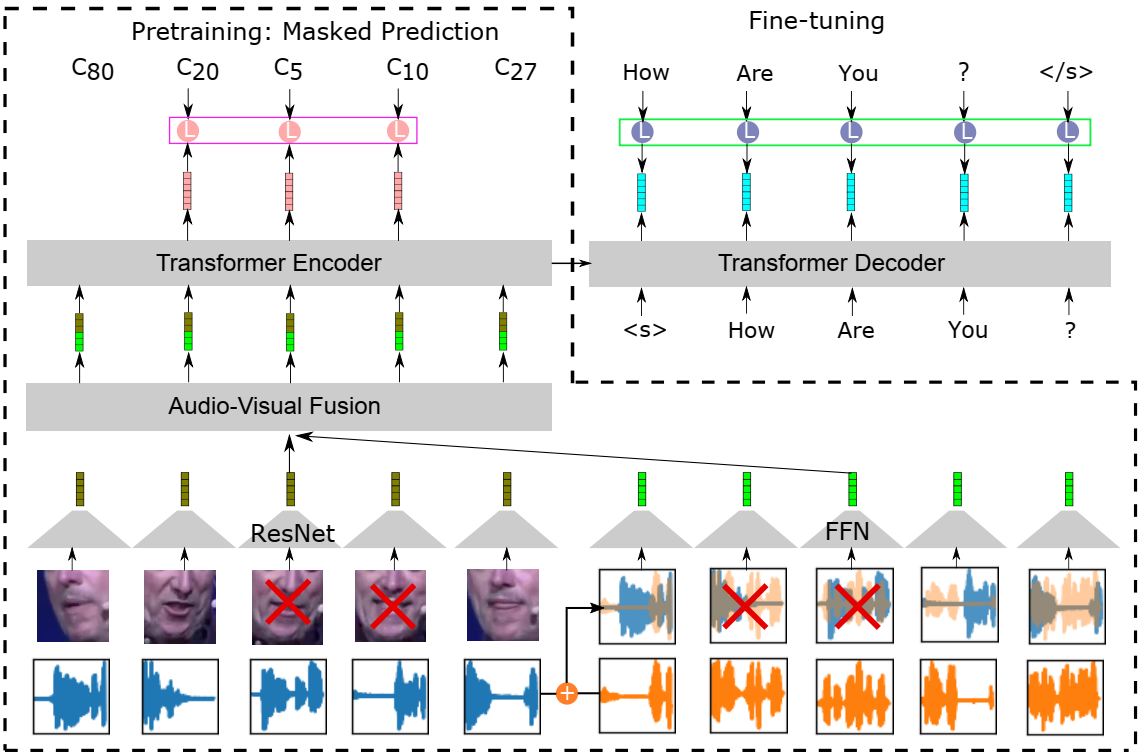
\includegraphics[width=\textwidth]{images/av-hubert-model}
	\caption[معماری مدل ای-وی هیوبرت]{معماری مدل ای-وی هیوبرت \cite{shi2022robust}}
	\label{fig:av-hubert-model}
\end{figure}

مدل ای-وی هیوبرت، بر پایه مدل هیوبرت ارائه شده است و رویکردی مشابه را این‌بار برای حل مساله بازشناسی گفتار به واسطه صوت و تصویر در پی می‌گیرد. همانطور که در تصویر 
\ref{fig:av-hubert-model}
مشاهده می‌شود، در این مدل فریم‌های صوتی و بصری ویدیو، به ترتیب به واسطه کدکننده صوتی و کدکننده بصری به یک بازنمایی متراکم
\LTRfootnote{Dense Representation}
تبدیل می‌شوند.

در کدکننده بصری، از یک مدل رزنت-هجده 
\LTRfootnote{ResNet-18}
شده است. مدل های رزنت، به جای ساختار ترتیبی لایه‌ها، دارای اتصالات خارج از ترتیب بوده که موجب کاهش مشکل محوشدن گرادیان
\LTRfootnote{Vanishing Gradient}
و به تبع آن، افزایش تعداد لایه‌های مدل می‌شود. این نوع از مدل‌ها، پیش از ارائه مدل‌های مبتنی بر ویژن‌ترنسفورمر
\LTRfootnote{Vision Transformer (ViT)}
، دارای بهترین عملکرد در حوزه تصویر بوده‌اند. پیش از ورودی دادن فریم‌های بصری ویدیو به این مدل رزنت-هجده، تغییرات زیر بر روی تصویر اعمال می شود.

\begin{itemize}
	\item ۶۸ نقطه کلیدی چهره تشخیص داده شده و سپس به واسطه یک تبدیل خطی، این نقاط کلیدی به یک دستگاه مختصات متمرکز بر چهره انتقال پیدا می‌کند.
	\item یک منطقه مورد علاقه
	\LTRfootnote{Region of Interest (ROI)}
	با ابعاد ۹۶×۹۶ حول دهان فرد در چهره بریده می‌شود.
	\item کانال‌های رنگی تصویر به سطح خاکستری منتقل می‌شوند.
	\item در جهت داده‌افزایی
	\LTRfootnote{Data Augmentation}
	یک کادر با ابعاد ۸۸×۸۸ به صورت تصادفی از منطقه مورد علاقه بریده شده و به صورت تصادفی به صورت افقی قرینه
	\LTRfootnote{Horizontal Flip}
	می شود.
\end{itemize}

به دلیل تاثیر بیشتر داده‌های صوتی نسبت به داده‌های بصری در این مساله، برای کاهش تاثیر داده‌های صوتی و افزایش تاثیر داده‌های بصری در یادگیری مدل، از یک شبکه تماما متصل عصبی استفاده شده است. فریم‌های صوتی خام ورودی، پیش از ورودی داده شدن به شبکه عصبی، به واسطه یک استخراج کننده ویژگی خاص
\LTRfootnote{Log Filterbank Energy}
به یک بردار ۲۶ بعدی با فاصله ۱۰ میلی‌ثانیه تبدیل می‌شود. علاوه بر این، به دلیل تفاوت نرخ برداشت فریم های صوتی و بصری - فریم‌های صوتی با فرکانس صد هرتز و فریم‌های بصری با فرکانس ۲۵ هرتز برداشت می‌شود - به ازای هر فریم بصری،چهار فریم صوتی برداشت می‌شود تا هماهنگی زمانی میان دو نوع داده حفظ شود.

پس از ایجاد یک بازنمایی متراکم از فریم‌های صوتی و بصری ویدیو، این بازنمایی به عنوان ورودی به لایه‌های کدکننده ترنسفورمر داده می‌شود. همانطور که در مدل زبانی برت و مدل بازشناسی گفتار هیوبرت توضیح داده شد، در اینجا نیز شبکه کدکننده به دنبال حدس آواهای پوشانده شده است و تلاش می‌کند با این کار، ماهیت و ارتباط میان آواها را به صورت بدون نظارت درک کند. در این مرحله، با استفاده از داده‌های بدون برچسب، می‌توان پیش‌آموزش
\LTRfootnote{Pre-Train}
مدل را انجام داد و در نهایت برای تکمیل فرایند یادگیری مدل و انتقال دانش کسب شده در فرایند پیش‌آموزش به مساله اصلی، مدل با استفاده از داده‌های برچسب‌خورده، کوک می‌شود. برای این انتقال دانش، از یک شبکه کدبرگردان
\LTRfootnote{Decoder}
ترنسفورمری به همراه تابع زیان سی-تی-سی
\LTRfootnote{Connectionist Temporal Classification Loss (CTC Loss)}
 استفاده می‌شود.
 
 \subsection{دادگان‌های صوتی-تصویری موجود}
 
 پیش از ارائه مدل‌های خود-نظارتی یا نیمه-نظارت‌شده، رویکرد غالب مدل‌ها در جهت حل مساله بازشناسی گفتار به واسطه صوت و تصویر، مبتنی بر مدل‌های نظارت‌شده بوده است. به همین دلیل، عملکرد و دقت این مدل‌ها به حجم دادگان وابسته بوده و در صورت محدود بودن آن، کیفیت و عملکرد پایینی از خود نشان می‌دادند.
 
 با توجه به این توضیحات، بررسی دادگان‌های موجود ضروری به نظر می‌رسد. در ادامه، به صورت مختصر شرحی در رابطه با مشخصات دادگان‌های ال-آر-اس دو و سه
 \LTRfootnote{LRS2-BBC, LRS3-TED}
و وکس-سلب
 \LTRfootnote{Vox-Celeb}
بیان خواهد شد.
   
\subsubsection{دادگان ال-آر-اس دو و سه}

دادگان ال-آر-اس دو، یکی از بزرگ‌ترین دادگان‌های موجود برای مساله لب‌خوانی می‌باشد. این دادگان با استفاده از برنامه‌های تلویزیونی - به ویژه اخبار و برنامه‌های گفتگومحور
\LTRfootnote{Talk Show}
- شبکه انگلیسی زبان بی-بی-سی
\LTRfootnote{BBC}
تشکیل شده است. پس از ارائه این دادگان، دادگان دیگری با نام ال-آر-اس سه، این‌بار با استفاده از ویدیو‌های سخنرانی‌های برنامه‌های تد
\LTRfootnote{TED}
و تد-ایکس
\LTRfootnote{TEDx}
توسط محققان دانشگاه آکسفورد
\LTRfootnote{Oxford University}
منتشر شد. این دو دادگان، از بزرگ‌ترین دادگان‌های برچسب‌گذاری شده به زبان انگلیسی می‌باشند و معیار ارزیابی
\LTRfootnote{Benchmark}
در مساله بازشناسی گفتار به واسطه صوت و تصویر محسوب می‌شوند.

\subsubsection{دادگان وکس-سلب}

 این دادگان، یک دادگان چند‌زبانه است که در ابتدا برای مساله تشخیص گوینده چندزبانه با استفاده از داده‌های صوتی و بصری ارائه شده است. بر روی هم، این دادگان شامل بیش از دو هزار و ۴۴۲ ساعت گفتار از بیش از شش هزار گوینده که از سایت اشتراک‌گذاری ویدیو یوتیوب
\LTRfootnote{YouTube}
استخراج شده است، می‌باشد. همچنین، این دادگان شامل زیرنویس و متن اصلی که در ویدیو‌ها بیان می‌شود، نمی‌باشد. مزیت این دادگان نسبت به دادگان ال-آر-اس دو و سه، تنوع بیشتر موقعیت‌ها و صحنه‌هایی است که وجود دارد. 
 
\subsection{ایجاد دادگان فارسی}

با توجه به توضیحات داده شده در بخش قبل، دادگان‌های موجود برای حل مساله بازشناسی گفتار به واسطه صوت و تصویر، غالبا به زبان انگلیسی بوده و در زبان فارسی قابل استفاده نمی‌باشند. به همین دلیل، در این دوره تصمیم به ایجاد و جمع‌آوری یک دادگان فارسی گرفتیم.

پیش از شروع فرایند جمع‌آوری ویدیو‌ها، مقالات متناظر با دادگان‌های ال-آر-اس سه و وکس-سلب را مطالعه کردم. با توجه به نکات ذکر شده در این مقالات، می‌بایست به سوالات زیر جواب داده می‌شد:

\begin{itemize}
	\item منبع جمع‌آوری ویدیو‌ها
	\item چگونگی استخراج ویدیو‌ها
	\item چگونگی پردازش ویدیو‌ها
	\item چگونگی فرایند برچسب‌زنی داده‌های استخراج‌شده
\end{itemize}

\subsubsection{منبع جمع‌آوری ویدیو‌ها}

با توجه به این موضوع که داده‌های دادگان‌های مطرح انگلیسی، با استفاده از برنامه‌های تلویزیونی و ویدیو‌های اشتراک گذاشته شده در سایت اشتراک‌گذاری ویدیو یوتیوب به دست آمده بودند، گزینه‌های زیر از گزینه‌های مطرح برای جمع‌آوری ویدیو‌های فارسی بودند:

\begin{itemize}
	\item سایت تلوبیون
	\item سایت آپارات
	\item سایت یوتیوب
	\item شبکه اجتماعی توییتر
	\LTRfootnote{Twitter}
	\item شبکه اجتماعی اینستاگرام
	\LTRfootnote{Instagram}
	\item سایت‌های آموزش ویدیویی نظیر فرادرس و مکتب‌خونه
\end{itemize}

در نهایت، از میان این گزینه‌ها، سایت تلوبیون به دلیل برخورداری از ویدیو‌های برنامه‌های تلویزیونی و نیازمندی به پالایش کمتر داده‌های این سایت، انتخاب شد. بنا به الگوگیری از دادگان ال-آر-اس دو و سه، در این مرحله تصمیم نهایی بر استخراج ویدیو‌های آرشیوی شبکه خبر صدا و سیما جمهوری اسلامی ایران شد.

در ادامه برای ارتقای این دادگان، می‌توان از داده‌های ویدیویی دیگر برنامه‌های تلویزیون به خصوص برنامه‌های گفتگومحور دیگر شبکه‌های صدا و سیما جمهوری اسلامی ایران نیز استفاده نمود، اما در این مرحله به دلیل محدود بودن زمان این عمل به نسخه‌های بعدی این دادگان موکول شده است.

\subsubsection{چگونگی استخراج ویدیو‌ها}

برای استخراج ویدیو‌های آرشیو تلویزیون از سایت تلوبیون، یک اسکریپت به زبان پایتون
\LTRfootnote{Python}
و با استفاده از کتابخانه سلنیوم
\LTRfootnote{Selenium}
توسعه داده شده است. زبان پایتون یکی از زبان‌های مفسری
\LTRfootnote{Interpreter}
مطرح می‌باشد. علاوه بر این، کتابخانه سلنیوم، اجازه استفاده به صورت خودکار از مرورگر را به توسعه‌دهندگان داده و توانایی خودکار سازی فرایند‌های مرورگر را با استفاده از زبان‌های برنامه‌نویسی دیگر می‌دهد.

از دیگر گزینه‌های مطرح برای انجام فرایند استخراج ویدیو‌ها، استفاده از کتابخانه ریکوئستز
\LTRfootnote{requests}
و بیوتیفول سوپ
\LTRfootnote{BeautifulSoup}
بوده است. با این حال، به دلیل بارگذاری کند
\LTRfootnote{Lazy Loading}
سایت تلوبیون، امکان استفاده از این کتابخانه‌ها وجود نداشت و به همین دلیل از کتابخانه سلنیوم برا انجام این کار استفاده شده است.

این اسکریپت با استفاده از یک برنامه راه‌اندازی
\LTRfootnote{Driver}
مربوط به مرورگر، با مرورگر متصل شده و سپس فرایند اتوماسیون و خودکار سازی را شروع می‌کند. این اسکرپیت در ابتدا، با توجه به ورودی تعیین شده به تعداد روز‌های تعیین شده، از آرشیو ویدیو‌های امروز شروع کرده و به تدریج به سراغ ویدیو‌های روز‌های قبل رفته و لینک‌های دانلود مربوط به هر ویدیو را استخراج کرده و در یک فایل متنی، ذخیره می‌کند. علاوه بر این، پس از استخراج لینک‌های دانلود ویدیو‌ها، توانایی شروع دانلود ویدیو‌ها را در اختیار دارد.

\subsubsection{چگونگی پردازش ویدیو‌ها}

ویدیو‌ها پس از دانلود، می‌بایست پردازش شده تا آماده ورودی داده شدن به مدل شوند. در این قسمت با بررسی اسکریپت‌های موجود به صورت عمومی، متوجه شدیم که خط لوله
\LTRfootnote{Pipeline}
پردازشی مربوط به دادگان وکس-سلب به صورت عمومی در سایت گیت‌هاب منتشر شده است و بدون تغییر قابل استفاده می‌باشد. این خط لوله، مربوط به مدل صوتی-تصویری سینک‌نت
\LTRfootnote{SyncNet}
می‌باشد که برای هماهنگ کردن حرکت لب‌های فرد گوینده و صوت استفاده می‌شود.

در این مدل، با استفاده از چارچوب پایتورچ و مدل‌های تشخیص چهره آماده با نام اس-سه-اف-دی
\LTRfootnote{S3FD}
چهره‌های موجود در تصویر تشخیص داده شده و در طول ویدیو دنبال می‌شوند. و در نهایت، تمامی چهره‌های موجود در ویدیو، به صورت ویدیو‌هایی از ویدیو اصلی جدا شده و برای استفاده در حل مسائل دیگر نظیر مساله بازشناسی گفتار به واسطه صوت و تصویر قابل استفاده می‌باشد. در تصویر 
\ref{fig:syncnet-sample}
چهار نمونه از خروجی‌های خط لوله پردازشی مدل سینک‌نت را مشاهده می‌کنید.

\begin{figure}[!h]
	\centering
	\captionsetup{justification=centering}
	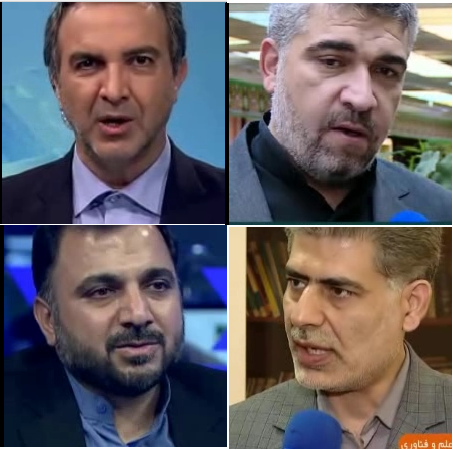
\includegraphics[width=9cm]{images/syncnet-sample}
	\caption{چهار نمونه از خروجی‌های خط لوله پردازشی مدل سینک‌نت}
	\label{fig:syncnet-sample}
\end{figure}

پیش از استفاده از این خط لوله پردازشی، به دنبال توسعه یک خط لوله از ابتدا بوده‌ام. برای این کار، ابتدا از مدل ام-تی-سی-ان-ان
\LTRfootnote{MTCNN}
که یک مدل تشخیص چهره با قابلیت آشکارسازی در یک صحنه
\LTRfootnote{Single Shot Detector (SSD)}
می‌باشد، استفاده کردم. این مدل قابلیت تشخیص چندین چهره در یک تصویر را داشته است. علاوه بر تشخیص کادر چهره فرد، قادر به تشخیص نقاط کلیدی چهره از جمله محل چشمان، محل لب و محل بینی فرد نیز بوده است.

با این حال، به دلیل دقت بالاتر و سادگی پیاده‌سازی خط لوله مربوط به مدل سینک‌نت، استفاده از این مدل آماده را برای پردازش نهایی ویدیو‌ها برگزیدم.

البته در فرایند پردازش ویدیو‌ها، دسته‌ای از خروجی‌های این مدل به اشتباه استخراج شده و نیازمند حذف در مرحله بعدی می‌باشند. حالت کلی این ویدیو‌های به اشتباه استخراج شده به شکل زیر می‌باشد:

\begin{itemize}
	\item ویدیو‌هایی که فرد صحبت نمی‌کند ولی به دلیل وجود گفتار پس‌زمینه به اشتباه استخراج شده است.
	\item ویدیو‌هایی که فرد گوینده، ماسک به صورت داشته است.
	\item ویدیو‌هایی که دارای صدای دوبله‌شده می‌باشد. برای نمونه ترجمه مترجم بر روی صحبت‌های یک فرد غیر فارسی زبان.
\end{itemize}

از آنجایی که این نوع از ویدیو‌های خروجی، از احتمال رخداد پایینی برخوردارند، می‌توان یکی از دو رویکرد زیر را در مواجهه با آنها در پیش گرفت:

\begin{itemize}
	\item تشخیص به صورت دستی و حذف آنها
	\item کوک کردن یک مدل به واسطه تمامی خروجی‌های مدل و تشخیص ویدیو‌های با ضریب اعتماد پایین
	\LTRfootnote{Low Confident}
\end{itemize}

با توجه به مشورت‌های انجام شده با منتور‌های این دوره، تصمیم نهایی بر این شد که رویکرد دوم اتخاذ شود. به گونه‌ای که در ابتدا تمام خروجی‌ها استخراج شده و پس از کوک کردن مدل نهایی، با یافتن ویدیو‌های با ضریب اعتماد پایین، این ویدیو‌ها بررسی شده و در صورتی که یکی از حالات ذکر شده در بالا باشند، حذف شوند.

علاوه بر این، به دلیل حجم بالای ویدیو‌های دانلود شده (حدود ۲۳۲ گیگابایت)، فرایند پردازش ویدیو به سادگی میسر نبوده است. با توجه به امکانات شرکت، سرور
\LTRfootnote{Server}
دارای کارت گرافیک
\LTRfootnote{GPU}
شرکت، دارای حافظه کافی برای انتقال کامل داده‌ها به این سرور و سپس پردازش تمامی آن‌ها وجود نداشت. به همین دلیل برای رفع این مشکل، از ارتباط میان سرور‌های شبکه به صورت محلی استفاده کرده و در هر مرحله، یک ویدیو را با استفاده از دستور اس-سی-پی
\LTRfootnote{scp}
از سرور دارای ویدیو‌ها دانلود‌شده به سرور فعلی منتقل کرده و پس از اعمال پردازش مربوطه بر روی این ویدیو، خروجی‌های میانی مربوط به این داده را در سرور پردازشی پاک کرده و خروجی نهایی را به سرور اولیه که دارای حجم ذخیره‌سازی کافی بوده است، ارسال می‌کردم. 

از آنجایی که فرایند پردازش ویدیو‌های دانلود شده فرایندی زمانبر می‌باشد و همچنین ارتباط شبکه محلی میان سرور‌های شرکت، دارای سرعت بالایی - حدود ۱ گیگابیت به ازای هر ثانیه - دارا می‌باشد، این عامل منجر به کندی تاثیر‌گذاری در سیستم نهایی نشده و قابل چشم‌پوشی می‌باشد.

\subsubsection{چگونگی فرایند برچسب‌زنی داده‌های استخراج‌شده}

داده‌های آموزشی مرتبط با مساله بازشناسی گفتار به واسطه صوت و تصویر، علاوه بر فریم‌های صوتی و بصری، نیازمند متن بیان شده در فریم‌های ویدیو نیز می‌باشند. به همین دلیل، نیاز است که پس از دانلود ویدیو‌ها و پردازش آنها، متن مرتبط با هر یک از این ویدیو‌ها استخراج شده و به عنوان برچسب این ویدیو مشخص شود. برای انجام فرایند برچسب‌زنی داده‌ها در دسترس، با توجه به مشاوره‌های انجام شده با منتور‌های دوره کارآموزی، راهکارهای زیر مطرح شده است:

\begin{itemize}
	\item جمع‌سپاری
	\LTRfootnote{Crowd Sourcing}
	داده‌های ویدیویی
	\item برچسب‌گذاری به صورت دستی توسط عوامل دوره کارآموزی
	\item استفاده از یک مدل آماده تبدیل گفتار به متن
	\LTRfootnote{Automatic Speech Recognition}
	و بررسی خروجی آن به ازای هر یک از ویدیو‌ها
\end{itemize}

با توجه به زمان محدود دوره کارآموزی، گزینه اول و دوم به دلیل زمانبر بودن، کنار گذاشته شده و تصمیم نهایی بر این شد که با استفاده از یک مدل تبدیل گفتار به متن و سپس بررسی خروجی این مدل به ازای هر ویدیو، این فرایند را سرعت بخشیده و دادگان را سریع‌تر آماده کرد.

در حال حاضر، حدود دو هزار و سیصد و نود ویدیو دانلود شده است و این تعداد ویدیو، در حال پردازش توسط خط لوله پردازشی سینک‌نت می‌باشد. به دلیل زمانبر بودن فرایند پردازشی، فعالیت فعلی در این پروژه تا به اینجا محدود شده است. پس از آماده سازی دادگان، امکان کوک کردن مدل ای-وی هیوبرت و دیگر مدل‌های آماده نیز وجود دارد و می‌توان میزان مفید بودن این دادگان فارسی جمع‌آوری شده را به طور بهتری ارزیابی کرد.

علاوه بر این، این دادگان قابل استفاده در مسائل دیگری نظیر تشخیص لب‌خوانی به زبان فارسی نیز می‌باشد و توانایی استفاده برای کوک کردن مدل‌های آماده موجود را نیز دارا می‌باشد.
%\chapter{نتیجه‌گیری و پیشنهاد‌ها}

در این فصل، در ابتدا به مرور نکات ذکر شده و جمع‌بندی آنها پرداخته و سپس پیشنهاد‌هایی در جهت بهبود و ارتقا سامانه و دادگان جمع‌آوری شده ارائه می‌شود.

\section{نتیجه‌گیری و جمع‌بندی}

همانطور که در فصل‌های قبل بررسی شد، استفاده از داده‌های تصویری حرکت لب‌های فرد گوینده، داده مناسبی برای جبران نقص در سیگنال‌های صوتی مربوط به گفتار می‌باشد. علاوه بر این، این مکانیزم در سیستم شنیداری انسان نیز وجود دارد و علاوه بر گوش‌ها، دیدن حرکت لب‌های گوینده نیز تاثیر به سزایی در فهم متن بیان شده توسط گوینده دارد.

همچنین، به دلیل محدود بودن داده‌های برچسب‌گذاری شده ویدیویی، استفاده از رویکرد‌های خود-نظارتی و نیمه-نظارت‌شده نسبت به رویکرد نظارت‌شده، عملکرد بهتری از خود نشان داده و از پایداری بهتری برخوردار خواهد بود. در این مدل‌ها، تلاش می‌شود که دانش کلی نسبت به ماهیت و ارتباط داده‌ها به دست آمده (در فرایند پیش‌آموزش بر روی داده‌های بدون برچسب) و سپس این دانش به طور خاص بر روی حل مساله مورد نظر کوک شود.

این رویکرد، رویکرد مناسبی برای استفاده در زبان‌هایی است که داده ویدیو کافی نداشته باشند؛ چراکه با وجود داده برچسب‌گذاری شده کم نیز، توانایی رسیدن به عملکرد و دقت مناسب را دارا می‌باشند. با این حال، در زبان فارسی داده ویدیویی مناسب برای این مساله موجود نمی‌باشد. به همین دلیل در این مقاله در پی این بر آمدیم تا دادگان ویدیویی فارسی با استفاده از ویدیو‌های آرشیو شبکه خبر صدا و سیما جمهوری اسلامی ایران جمع‌آوری کنیم.


\section{پیشنهاد‌ها}

از جمله پیشنهاد‌هایی که می‌توان در جهت بهبود دادگان فعلی داد، استفاده از ویدیو برنامه‌های گفتگومحور دیگر شبکه‌های صدا و سیما جمهوری اسلامی ایران می‌باشد. علاوه بر این در صورت توسعه یک خط لوله پردازشی دقیق‌تر برای حذف خروجی‌های اشتباه مدل سینک‌نت، می‌توان به دادگان با کیفیت بالاتری دست یافت. این دادگان به دلیل حجم تخمینی کمی که دارد، برای فرایند کوک کردن مدل‌های بازشناسی گفتار به کمک صوت و تصویر، مناسب می‌باشد اما برای اجرای فرایند پیش‌آموزش مناسب نمی‌باشد. یکی از دیگر پیشنهاد‌ها در جهت بهبود این دادگان، استفاده از دیگر سایت‌های اشتراک‌گذاری ویدیو آنلاین نظیر آپارات، فرادرس و مکتب‌خونه می‌باشد.


%\include{chapter4}
%\include{chapter5}

%--------------------------------------------------------------------------appendix( مراجع و پیوست ها)
\chapterfont{\vspace*{-2em}\centering\LARGE}%

\appendix
\bibliographystyle{unsrt-fa}
\bibliography{references}
%\chapter*{‌پیوست}
\markboth{پیوست}{}
\addcontentsline{toc}{chapter}{پیوست}

لیست مقالات مرتبط با مساله بازشناسی گفتار به واسطه صوت و تصویر

\href{https://docs.google.com/spreadsheets/d/1Zdd84vojLO7jm_wr2Aev-HX1QdLINjyfSPAFpuWEYVs/edit?usp=sharing}{لینک دسترسی به برگه گوگل مقالات جمع‌آوری شده}
%--------------------------------------------------------------------------dictionary(واژه نامه ها)
%اگر مایل به داشتن صفحه واژه‌نامه نیستید، خط زیر را غیر فعال کنید.
\parindent=0pt
%%
\chapter*{واژه‌نامه‌ی فارسی به انگلیسی}
\pagestyle{style9}

\addcontentsline{toc}{chapter}{واژه‌نامه‌ی فارسی به انگلیسی}
%%%%%%
\begin{multicols*}{2}

{\bf آ}
\vspace*{3mm}


\farsiTOenglish{اسکالر}{Scalar}


\vspace*{3mm}
{\bf ب}
\vspace*{3mm}

\farsiTOenglish{بالابر}{Lift}


\vspace*{3mm}
{\bf پ}
%%\vspace*{3mm}

\farsiTOenglish{پایا}{Invariant}



\vspace*{3mm}
{\bf ت}
%%\vspace*{3mm}

\farsiTOenglish{ تناظر }{Correspondence}


\vspace*{3mm}
{\bf ث}
%%\vspace*{3mm}

\farsiTOenglish{ثابت‌ساز}{Stabilizer}

\vspace*{3mm}
{\bf ج}
%%\vspace*{3mm}

\farsiTOenglish{جایگشت}{Permutation}



\vspace*{3mm}
{\bf چ}
%%\vspace*{3mm}


\farsiTOenglish{چند جمله‌ای }{Polynomial}

\vspace*{3mm}
{\bf ح}
%%\vspace*{3mm}

\farsiTOenglish{حاصل‌ضرب دکارتی}{Cartesian product}


\vspace*{3mm}
{\bf خ}
%%\vspace*{3mm}

\farsiTOenglish{خودریختی}{Automorphism}

\vspace*{3mm}
{\bf د}
%%\vspace*{3mm}

\farsiTOenglish{درجه}{Degree}


\vspace*{3mm}
{\bf ر}
%%\vspace*{3mm}


\farsiTOenglish{ریزپردازنده}{microprocessor}


\vspace*{3mm}
{\bf ز}
%%\vspace*{3mm}


\farsiTOenglish{زیرمدول}{Submodule}


\vspace*{3mm}
{\bf س}
%%\vspace*{3mm}

\farsiTOenglish{سرشت}{Character}


\vspace*{3mm}
{\bf ص}
%%\vspace*{3mm}

\farsiTOenglish{صادقانه}{Faithful}

\vspace*{3mm}
{\bf ض}
%%\vspace*{3mm}

\farsiTOenglish{ضرب داخلی}{Inner product}

\vspace*{3mm}
{\bf ط}
%%\vspace*{3mm}


\farsiTOenglish{طوقه}{Loop}


\vspace*{3mm}
{\bf ظ}
%%\vspace*{3mm}


\farsiTOenglish{ظرفیت}{Valency}
 
\vspace*{3mm}
{\bf ع}
%%\vspace*{3mm}


\farsiTOenglish{عدم مجاورت}{Nonadjacency}



\vspace*{3mm}
{\bf ف}
%%\vspace*{3mm}

\farsiTOenglish{فضای برداری}{Vector space}



\vspace*{3mm}
{\bf ک}
%%\vspace*{3mm}

\farsiTOenglish{کاملاً تحویل‌پذیر}{Complete reducibility}


\vspace*{3mm}
{\bf گ}
%%\vspace*{3mm}


\farsiTOenglish{گراف}{Graph}



\vspace*{3mm}
{\bf م}
%%\vspace*{3mm}

\farsiTOenglish{ماتریس جایگشتی}{Permutation matrix }


\vspace*{3mm}
{\bf ن}
%%\vspace*{3mm}

\farsiTOenglish{ناهمبند}{Disconnected}


\vspace*{3mm}
{\bf و}
%%\vspace*{3mm}

\farsiTOenglish{وارون‌پذیر}{Invertible}


\vspace*{3mm}
{\bf ه}
%%\vspace*{3mm}

\farsiTOenglish{همبند}{Connected}



\vspace*{3mm}
{\bf ی}
%%\vspace*{3mm}

\farsiTOenglish{یال}{Edge}




\end{multicols*}
%%%%%%%
\chapter*{ واژه‌نامه‌ی انگلیسی به فارسی}
\pagestyle{style9}
\lhead{\thepage}\rhead{واژه‌نامه‌ی انگلیسی به فارسی}
\addcontentsline{toc}{chapter}{واژه‌نامه‌ی انگلیسی به فارسی}

\LTRmulticolcolumns
\begin{multicols}{2}
{\hfill\bf  \lr{A}}
%%\vspace*{1.5mm}

\englishTOfarsi{Automorphism}{خودریختی}

\vspace*{3mm}
{\hfill\bf   \lr{B}}
%%\vspace*{1.5mm}

\englishTOfarsi{Bijection}{دوسویی}

\vspace*{3mm}
{\hfill\bf   \lr{C}}
%%\vspace*{1.5mm}

\englishTOfarsi{Cycle group}{گروه دوری}

\vspace*{3mm}
{\hfill\bf   \lr{D}}
%%\vspace*{1.5mm}

\englishTOfarsi{Degree}{درجه}

\vspace*{3mm}
{\hfill\bf   \lr{E}}
%%\vspace*{1.5mm}

\englishTOfarsi{Edge}{یال}

\vspace*{3mm}
{\hfill\bf   \lr{F}}
%%\vspace*{1.5mm}

\englishTOfarsi{Function}{تابع}

\vspace*{3mm}
{\hfill\bf   \lr{G}}
%%\vspace*{1.5mm}

\englishTOfarsi{Group}{گروه}

\vspace*{3mm}
{\hfill\bf   \lr{H}}
%%\vspace*{1.5mm}

\englishTOfarsi{Homomorphism}{همریختی}

\vspace*{3mm}
{\hfill\bf   \lr{I}}
%%\vspace*{1.5mm}

\englishTOfarsi{Invariant}{پایا}

\vspace*{3mm}
{\hfill\bf   \lr{L}}
%%\vspace*{1.5mm}

\englishTOfarsi{Lift}{بالابر}

\vspace*{3mm}
{\hfill\bf   \lr{M}}
%%\vspace*{1.5mm}

\englishTOfarsi{Module}{مدول}

\vspace*{3mm}
{\hfill\bf   \lr{N}}
%%\vspace*{1.5mm}

\englishTOfarsi{Natural map}{نگاشت طبیعی}

\vspace*{3mm}
{\hfill\bf   \lr{O}}
%%\vspace*{1.5mm}

\englishTOfarsi{One to One}{یک به یک}

\vspace*{3mm}
{\hfill\bf   \lr{P}}
%%\vspace*{1.5mm}

\englishTOfarsi{Permutation group}{گروه جایگشتی}

\vspace*{3mm}
{\hfill\bf   \lr{Q}}
%%\vspace*{1.5mm}

\englishTOfarsi{Quotient graph}{گراف خارج‌قسمتی}

 \vspace*{3mm}
{\hfill\bf   \lr{R}}
%%\vspace*{1.5mm}

\englishTOfarsi{Reducible}{تحویل پذیر}

\vspace*{3mm}
{\hfill\bf   \lr{S}}
%%\vspace*{1.5mm}

\englishTOfarsi{Sequence}{دنباله}

 \vspace*{3mm}
{\hfill\bf   \lr{T}}
%%\vspace*{1.5mm}

\englishTOfarsi{Trivial character}{سرشت بدیهی}

\vspace*{3mm}
{\hfill\bf   \lr{U}}
%%\vspace*{1.5mm}

\englishTOfarsi{Unique}{منحصربفرد}

\vspace*{3mm}
{\hfill\bf   \lr{V}}
%%\vspace*{1.5mm}

\englishTOfarsi{Vector space}{فضای برداری}
\end{multicols}
%--------------------------------------------------------------------------index(نمایه)
%اگر مایل به داشتن صفحه نمایه نیستید، خط زیر را غیر فعال کنید.
%\pagestyle{style7}
%\printindex
%\pagestyle{style7}
%%کلمات کلیدی انگلیسی
\latinkeywords{Write a 3 to 5 KeyWords is essential. Example: AUT, M.Sc., Ph. D,..}
%چکیده انگلیسی

\en-abstract{
This page is accurate translation from Persian abstract into English.
}
%%%%%%%%%%%%%%%%%%%%% کدهای زیر را تغییر ندهید.

\newpage
\thispagestyle{empty}
\begin{latin}
\section*{\LARGE\centering Abstract}

\een-abstract

\vspace*{.5cm}
{\large\textbf{Key Words:}}\par
\vspace*{.5cm}
\elatinkeywords
\end{latin}
%% در این فایل، عنوان پایان‌نامه، مشخصات خود و چکیده پایان‌نامه را به انگلیسی، وارد کنید.
%%%%%%%%%%%%%%%%%%%%%%%%%%%%%%%%%%%%
\baselineskip=.6cm
\begin{latin}

\latinfaculty{Department of ...}


\latintitle{Title of Thesis}


\firstlatinsupervisor{Dr. }

%\secondlatinsupervisor{Second Supervisor}

\firstlatinadvisor{Dr. }

%\secondlatinadvisor{Second Advisor}

\latinname{Name}

\latinsurname{Surname}

\latinthesisdate{Month \& Year}

\latinvtitle
\end{latin}

\end{document}
